%md->tex->template
\documentclass[12pt]{article}
\usepackage{CJKutf8}
\usepackage{amsmath}
\usepackage{geometry}
\usepackage{fancyhdr}
\usepackage{longtable,booktabs}
\usepackage{enumerate}
\usepackage{enumitem}
\usepackage{amsthm}
\usepackage{amssymb}
\usepackage{tikz}
\setlist[enumerate,1]{font=\bfseries}
\geometry{left=3.0cm,right=2.0cm,top=3.0cm,bottom=3.0cm}

\newenvironment{firstlayer}%
{\begin{list}{}{\renewcommand{\makelabel}[1]{\textbf{##1}.\hfil}
}}
{\end{list}}
\newenvironment{secondlayer}%
{\begin{list}{}{\renewcommand{\makelabel}[1]{(##1)\hfil}
}}
{\end{list}}

\renewcommand{\proofname}{\textbf{证明}}

\providecommand{\sol}{\textbf{解}.~}

\title{第 11 次作业}
\author{Log Creative}
\date{May 23, 2020}
\begin{document}

\begin{CJK}{UTF8}{gbsn}

\maketitle

\begin{firstlayer}
  \item[17] 对$A$上的关系$R$,证明:
  \begin{secondlayer}
    \item[1] $R$是自反的$\Leftrightarrow I_A\subseteq R$
    \begin{proof}
      $R$是自反的$\Rightarrow \forall\langle x,y\rangle\in I_A\Leftrightarrow x=y\Rightarrow \langle x,y \rangle\in R\Rightarrow I_A\subseteq R$

$I_A\subseteq R\Rightarrow \forall x\in A,\langle x,x\rangle\in R\Rightarrow R$是自反的。

综上所述,$R$是自反的$\Leftrightarrow I_A\subseteq R$。
    \end{proof}
    \item[2]$R$是非自反的$\Leftrightarrow I_A\cap R=\varnothing$
    \begin{proof}
      $R$是非自反的$\Rightarrow \forall\langle x,y\rangle\in I_A\Leftrightarrow x=y\Rightarrow \langle x,y \rangle\notin R\Rightarrow I_A\cap R=\varnothing$

$I_A\cap R=\varnothing\Rightarrow \forall\langle x,x\rangle\in I_A,\langle x,x \rangle\notin R\Rightarrow R$是非自反的。

综上所述,$R$是非自反的$\Leftrightarrow I_A\cap R=\varnothing$。
    \end{proof}
    \item[3]$R$是传递的$\Leftrightarrow R\circ R\subseteq R$
    \begin{proof}
      $R$是传递的$\Rightarrow \forall\langle x,z\rangle\in R\circ R,\exists y\in A:\langle x,y\rangle\in R\wedge\langle y,z\rangle\in R\Rightarrow\langle x,z\rangle\in R\Rightarrow R\circ R\subseteq R$

$R\circ R\subseteq R\Rightarrow \forall\langle x,z\rangle\in R\circ R\subseteq R,\exists y\in A:\langle x,y\rangle\in R\wedge\langle y,z\rangle\in R\Rightarrow R$是传递的。
    \end{proof}
  \end{secondlayer}
  \item[22]对集合$A=\{a,b,c,d\}$上的两个关系
  \begin{align*}
    R_1&=\{\langle a,a \rangle,\langle a,b\rangle,\langle b,d \rangle\}\\
    R_2&=\{\langle a,d \rangle,\langle b,c \rangle,\langle b,d \rangle,\langle c,b \rangle\}
  \end{align*}
  求$R_1\circ R_2,R_2\circ R_1,R_1^2,R_2^2$。
  
  \sol \begin{align*}
         R_1\circ R_2&=\{\langle c,d\rangle\}\\
R_2\circ R_1&=\{\langle a,d \rangle,\langle a,c \rangle,\langle a,d \rangle \}\\
R_1^2&=\{ \langle a,a \rangle,\langle a,d \rangle ,\langle a,b \rangle\}\\
R_2^2&=\{\langle b,b  \rangle, \langle c,c \rangle,\langle c,d \rangle \}
       \end{align*}
    \item[24]$A=\{a,b,c,d,e\}$上的关系$R$的关系如图,给出$r(R),s(R),t(R)$的关系图。

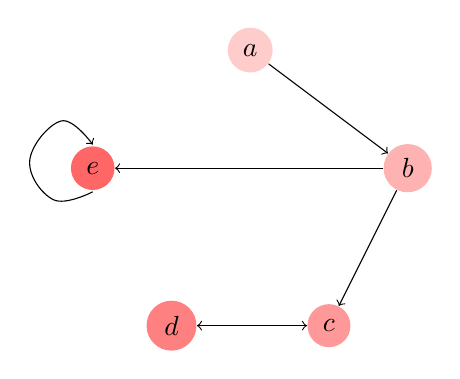
\begin{tikzpicture}

\node[circle, fill=red!20] (v1) at (-0.5,2.5) {$a$}  ;
\node[circle, fill=red!30] (v2) at (1.5,1) {$b$};
\node[circle, fill=red!40] (v3) at (0.5,-1) {$c$};
\node[circle, fill=red!50] (v4) at (-1.5,-1) {$d$};
\node[circle, fill=red!60] (v5) at (-2.5,1) {$e$};

\draw[->]  (v1) edge (v2);
\draw[->]   (v2) edge (v3);
\draw[->]  (v3) edge (v4);
\draw[->]  (v4) edge (v3);
\draw[->]  (v2) edge (v5);

% \draw[->]  (v5) edge (v4);
% \draw[->]  (v3) edge (v1);
% \draw[->]  (v4) edge (v2);
% \draw[->]  (v5) edge (v3);
%还差5个自环


%\draw[->]  plot[smooth, tension=.9] coordinates {(-0.8,2.5) (-1,3) (-0.5,3.4) (0,3) (-0.2,2.5)};
%\draw[->]  plot[smooth, tension=.9] coordinates {(1.5,1.3) (1.9,1.5) (2.3,1) (1.9,0.5) (1.5,0.7)};
%\draw[->]  plot[smooth, tension=.7] coordinates {(0.8,-0.9) (1.2,-1.1) (1.1,-1.6) (0.6,-1.7) (0.4,-1.3)};
%\draw[->]  plot[smooth, tension=.7] coordinates {(-1.3,-1.2) (-1.1,-1.6) (-1.7,-1.9) (-2.1,-1.4) (-1.8,-1.1)};
\draw[->]  plot[smooth, tension=.7] coordinates {(-2.5,0.7) (-3,0.6) (-3.3,1.1) (-2.9,1.6) (-2.5,1.3)};

\end{tikzpicture}

    \sol 
    
    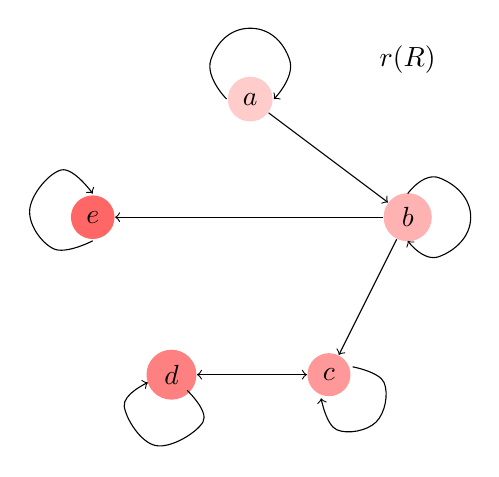
\begin{tikzpicture}

\node[circle, fill=red!20] (v1) at (-0.5,2.5) {$a$}  ;
\node[circle, fill=red!30] (v2) at (1.5,1) {$b$};
\node[circle, fill=red!40] (v3) at (0.5,-1) {$c$};
\node[circle, fill=red!50] (v4) at (-1.5,-1) {$d$};
\node[circle, fill=red!60] (v5) at (-2.5,1) {$e$};

\draw[->]  (v1) edge (v2);
\draw[->]   (v2) edge (v3);
\draw[->]  (v3) edge (v4);
\draw[->]  (v4) edge (v3);
\draw[->]  (v2) edge (v5);

% \draw[->]  (v5) edge (v4);
% \draw[->]  (v3) edge (v1);
% \draw[->]  (v4) edge (v2);
% \draw[->]  (v5) edge (v3);
%还差5个自环


\draw[->]  plot[smooth, tension=.9] coordinates {(-0.8,2.5) (-1,3) (-0.5,3.4) (0,3) (-0.2,2.5)};
\draw[->]  plot[smooth, tension=.9] coordinates {(1.5,1.3) (1.9,1.5) (2.3,1) (1.9,0.5) (1.5,0.7)};
\draw[->]  plot[smooth, tension=.7] coordinates {(0.8,-0.9) (1.2,-1.1) (1.1,-1.6) (0.6,-1.7) (0.4,-1.3)};
\draw[->]  plot[smooth, tension=.7] coordinates {(-1.3,-1.2) (-1.1,-1.6) (-1.7,-1.9) (-2.1,-1.4) (-1.8,-1.1)};
\draw[->]  plot[smooth, tension=.7] coordinates {(-2.5,0.7) (-3,0.6) (-3.3,1.1) (-2.9,1.6) (-2.5,1.3)};

\node at (1.5,3) {$r(R)$};
\end{tikzpicture}

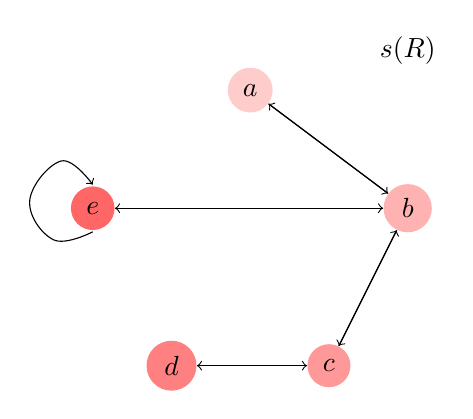
\begin{tikzpicture}

\node[circle, fill=red!20] (v1) at (-0.5,2.5) {$a$}  ;
\node[circle, fill=red!30] (v2) at (1.5,1) {$b$};
\node[circle, fill=red!40] (v3) at (0.5,-1) {$c$};
\node[circle, fill=red!50] (v4) at (-1.5,-1) {$d$};
\node[circle, fill=red!60] (v5) at (-2.5,1) {$e$};

\draw[->]  (v1) edge (v2);
\draw[->]  (v2) edge (v1);
\draw[->]   (v2) edge (v3);
\draw[->]   (v3) edge (v2);
\draw[->]  (v3) edge (v4);
\draw[->]  (v4) edge (v3);
\draw[->]  (v2) edge (v5);
\draw[->]  (v5) edge (v2);

% \draw[->]  (v5) edge (v4);
% \draw[->]  (v3) edge (v1);
% \draw[->]  (v4) edge (v2);
% \draw[->]  (v5) edge (v3);
%还差5个自环


%\draw[->]  plot[smooth, tension=.9] coordinates {(-0.8,2.5) (-1,3) (-0.5,3.4) (0,3) (-0.2,2.5)};
%\draw[->]  plot[smooth, tension=.9] coordinates {(1.5,1.3) (1.9,1.5) (2.3,1) (1.9,0.5) (1.5,0.7)};
%\draw[->]  plot[smooth, tension=.7] coordinates {(0.8,-0.9) (1.2,-1.1) (1.1,-1.6) (0.6,-1.7) (0.4,-1.3)};
%\draw[->]  plot[smooth, tension=.7] coordinates {(-1.3,-1.2) (-1.1,-1.6) (-1.7,-1.9) (-2.1,-1.4) (-1.8,-1.1)};
\draw[->]  plot[smooth, tension=.7] coordinates {(-2.5,0.7) (-3,0.6) (-3.3,1.1) (-2.9,1.6) (-2.5,1.3)};

\node at (1.5,3) {$s(R)$};
\end{tikzpicture}

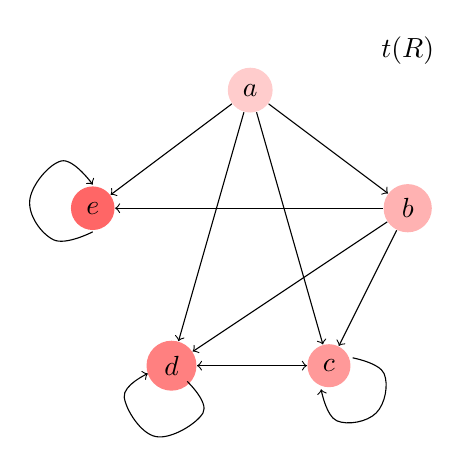
\begin{tikzpicture}

\node[circle, fill=red!20] (v1) at (-0.5,2.5) {$a$}  ;
\node[circle, fill=red!30] (v2) at (1.5,1) {$b$};
\node[circle, fill=red!40] (v3) at (0.5,-1) {$c$};
\node[circle, fill=red!50] (v4) at (-1.5,-1) {$d$};
\node[circle, fill=red!60] (v5) at (-2.5,1) {$e$};

\draw[->]  (v1) edge (v2);
\draw[->]   (v2) edge (v3);
\draw[->]  (v1) edge (v3);
\draw[->]  (v3) edge (v4);
\draw[->]  (v2) edge (v4);
\draw[->]  (v4) edge (v3);
\draw[->]  (v2) edge (v5);
\draw[->]  (v1) edge (v5);
\draw[->]  (v1) edge (v4);
% \draw[->]  (v5) edge (v4);
% \draw[->]  (v3) edge (v1);
% \draw[->]  (v4) edge (v2);
% \draw[->]  (v5) edge (v3);
%还差5个自环


%\draw[->]  plot[smooth, tension=.9] coordinates {(-0.8,2.5) (-1,3) (-0.5,3.4) (0,3) (-0.2,2.5)};
%\draw[->]  plot[smooth, tension=.9] coordinates {(1.5,1.3) (1.9,1.5) (2.3,1) (1.9,0.5) (1.5,0.7)};
\draw[->]  plot[smooth, tension=.7] coordinates {(0.8,-0.9) (1.2,-1.1) (1.1,-1.6) (0.6,-1.7) (0.4,-1.3)};
\draw[->]  plot[smooth, tension=.7] coordinates {(-1.3,-1.2) (-1.1,-1.6) (-1.7,-1.9) (-2.1,-1.4) (-1.8,-1.1)};
\draw[->]  plot[smooth, tension=.7] coordinates {(-2.5,0.7) (-3,0.6) (-3.3,1.1) (-2.9,1.6) (-2.5,1.3)};

\node at (1.5,3) {$t(R)$};
\end{tikzpicture}
\item[27] 对$A=\{a,b,c,d\}$上的关系
\begin{equation*}
  R=\{\langle a,b \rangle,\langle b,a \rangle,\langle b,c \rangle,\langle c,d \rangle\}
\end{equation*}
\begin{secondlayer}
  \item[1]分别用矩阵运算和作图法计算求$r(R),s(R)$和$t(R)$。
  \item[2]用 Warshall 算法求 $t(R)$。
  
\end{secondlayer}

  \sol \begin{secondlayer}
         \item[1] $M(R)=\left(\begin{matrix}
    0 & 1 & 0 & 0 \\
    1 & 0 & 1 & 0 \\
    0 & 0 & 0 & 1 \\
    0 & 0 & 0 & 0
\end{matrix}\right)$

$M(r(R))=M(R\cup R^0)=M(R)+ M(R^0)=\left(\begin{matrix}
    0 & 1 & 0 & 0 \\
    1 & 0 & 1 & 0 \\
    0 & 0 & 0 & 1 \\
    0 & 0 & 0 & 0
\end{matrix}\right)+\left(\begin{matrix}
    1 & 0 & 0 & 0 \\
    0 & 1 & 0 & 0 \\
    0 & 0 & 1 & 0 \\
    0 & 0 & 0 & 1
\end{matrix}\right)=\left(\begin{matrix}
    1 & 1 & 0 & 0 \\
    1 & 1 & 1 & 0 \\
    0 & 0 & 1 & 1 \\
    0 & 0 & 0 & 1
\end{matrix}\right)$

\begin{center}
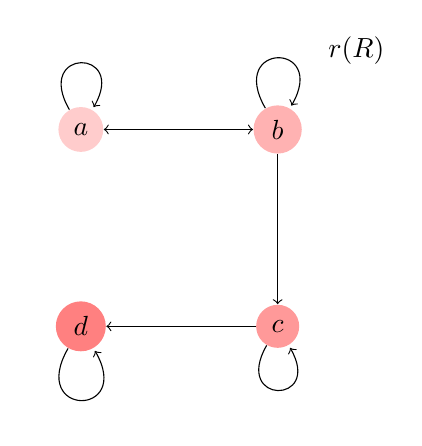
\begin{tikzpicture}

\node[circle, fill=red!20] (v1) at (-0.5,2.5) {$a$} edge [in=60,out=120,loop] ();
\node[circle, fill=red!30] (v2) at (2,2.5) {$b$} edge [in=60,out=120,loop] ();
\node[circle, fill=red!40] (v3) at (2,0) {$c$} edge [in=-60,out=-120,loop] ();
\node[circle, fill=red!50] (v4) at (-0.5,0) {$d$} edge [in=-60,out=-120,loop] ();

\node at (3,3.5) {$r(R)$};
\draw[->]  (v1) edge (v2);
\draw[->]  (v2) edge (v1);
\draw[->]  (v2) edge (v3);
\draw[->]  (v3) edge (v4);
\end{tikzpicture}
\end{center}
$M(R)+M(R^{-1})=\left(\begin{matrix}
    0 & 1 & 0 & 0 \\
    1 & 0 & 1 & 0 \\
    0 & 0 & 0 & 1 \\
    0 & 0 & 0 & 0
\end{matrix}\right) + \left(\begin{matrix}
    0 & 1 & 0 & 0 \\
    1 & 0 & 0 & 0 \\
    0 & 1 & 0 & 0 \\
    0 & 0 & 1 & 0
\end{matrix}\right)=\left(\begin{matrix}
    0 & 2 & 0 & 0 \\
    2 & 0 & 1 & 0 \\
    0 & 1 & 0 & 1 \\
    0 & 0 & 1 & 0
\end{matrix}\right)$

$M(s(R))=M(R\cup R^{-1})=\left(\begin{matrix}
    0 & 1 & 0 & 0 \\
    1 & 0 & 1 & 0 \\
    0 & 1 & 0 & 1 \\
    0 & 0 & 1 & 0
\end{matrix}\right)$

\begin{center}
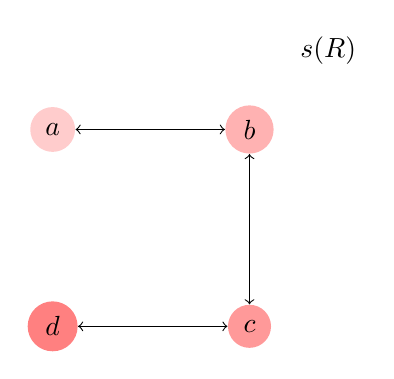
\begin{tikzpicture}

\node[circle, fill=red!20] (v1) at (-0.5,2.5) {$a$};
\node[circle, fill=red!30] (v2) at (2,2.5) {$b$};
\node[circle, fill=red!40] (v3) at (2,0) {$c$};
\node[circle, fill=red!50] (v4) at (-0.5,0) {$d$};

\node at (3,3.5) {$s(R)$};
\draw[->]  (v1) edge (v2);
\draw[->]  (v2) edge (v1);
\draw[->]  (v2) edge (v3);
\draw[->]  (v3) edge (v2);
\draw[->]  (v3) edge (v4);
\draw[->]  (v4) edge (v3);
\end{tikzpicture}
\end{center}

$M(t(R))=M(R\cup R^2 \cup R^3 \cup \cdots )=M(R)\vee M(R^2) \vee M(R^3) \vee \cdots=\left(\begin{matrix}
    0 & 1 & 0 & 0 \\
    1 & 0 & 1 & 0 \\
    0 & 0 & 0 & 1 \\
    0 & 0 & 0 & 0
\end{matrix}\right)\vee\left(\begin{matrix}
    1 & 0 & 1 & 0 \\
    0 & 1 & 0 & 1 \\
    0 & 0 & 0 & 0 \\
    0 & 0 & 0 & 0
\end{matrix}\right)\vee\left(\begin{matrix}
    0 & 1 & 0 & 1 \\
    1 & 0 & 1 & 0 \\
    0 & 0 & 0 & 0 \\
    0 & 0 & 0 & 0
\end{matrix}\right)\vee \cdots=\left(\begin{matrix}
    1 & 1 & 1 & 1 \\
    1 & 1 & 1 & 1 \\
    0 & 0 & 0 & 1 \\
    0 & 0 & 0 & 0
\end{matrix}\right)$

\begin{center}
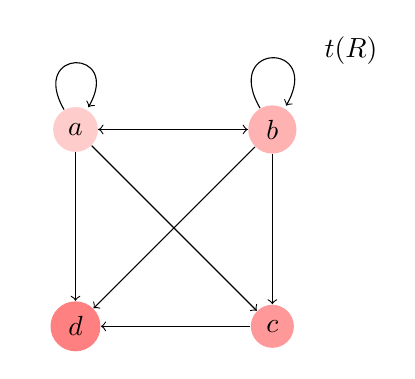
\begin{tikzpicture}

\node[circle, fill=red!20] (v1) at (-0.5,2.5) {$a$} edge [in=60,out=120,loop] ();
\node[circle, fill=red!30] (v2) at (2,2.5) {$b$} edge [in=60,out=120,loop] ();
\node[circle, fill=red!40] (v3) at (2,0) {$c$};
\node[circle, fill=red!50] (v4) at (-0.5,0) {$d$};

\node at (3,3.5) {$t(R)$};
\draw[->]  (v1) edge (v2);
\draw[->]  (v2) edge (v1);
\draw[->]  (v1) edge (v3);
\draw[->]  (v1) edge (v4);
\draw[->]  (v2) edge (v3);
\draw[->]  (v3) edge (v4);
\draw[->]  (v2) edge (v4);

\end{tikzpicture}
\end{center}
        \item[2]
        \begin{equation*}
          W_1=\left(\begin{matrix}
    0 & 1 & 0 & 0 \\
    1 & 1 & 1 & 0 \\
    0 & 0 & 0 & 1 \\
    0 & 0 & 0 & 0
\end{matrix}\right)
        \end{equation*}
        \begin{equation*}
          W_2=\left(\begin{matrix}
    1 & 1 & 1 & 0 \\
    1 & 1 & 1 & 0 \\
    0 & 0 & 0 & 1 \\
    0 & 0 & 0 & 0
\end{matrix}\right)
        \end{equation*}
        \begin{equation*}
          W_3=\left(\begin{matrix}
    1 & 1 & 1 & 1 \\
    1 & 1 & 1 & 1 \\
    0 & 0 & 0 & 1 \\
    0 & 0 & 0 & 0
\end{matrix}\right)
        \end{equation*}
        \begin{equation*}
          W_4=\left(\begin{matrix}
    1 & 1 & 1 & 1 \\
    1 & 1 & 1 & 1 \\
    0 & 0 & 0 & 1 \\
    0 & 0 & 0 & 0
\end{matrix}\right)=M(R^+)=M(t(R))
        \end{equation*}
       \end{secondlayer}
\end{firstlayer}

\end{CJK}

\end{document}

